

\chapter{Defensa frente a ataques adversarios} % Main chapter title

\label{Defensa} % Change X to a consecutive number; for referencing this chapter elsewhere, use \ref{ChapterX}

%----------------------------------------------------------------------------------------
%	SECTION 1
%----------------------------------------------------------------------------------------
A la fecha en que se redacta este documento no existe una solución definitiva que permita blindar completamente a una red neuronal de los ataques presentados en el presente documento. Las siguientes son las dificultades que enfrenta la elaboración y diseño de defensas \parencite{r7}:
\begin{itemize}
    \item La elaboración de un ejemplo adversario es un proceso de optimización complejo que no es lineal ni convexo para la mayoría de los modelos de aprendizaje automático. La falta de herramientas teóricas adecuadas para describir la solución a estos complejos problemas de optimización hace que sea aún más difícil hacer cualquier argumento teórico de que una defensa particular es robusta frente a un conjunto de ejemplos adversarios.

    \item Las técnicas de aprendizaje automático están diseñadas para entregar respuesta a cada entrada. Una modificación considerable del modelo para incorporar robustez frente a los ejemplos adversarios puede cambiar el objetivo elemental del modelo.
\end{itemize}
Lo anterior ha provocado un juego cíclico entre el atacante y el defensor del clasificador \parencite{r49}. Por ejemplo, en un sistema de filtro de correos no deseados, el atacante con el fin de hacer fallar la detección añade nuevas palabras al correo. Cuando el defensor se da cuenta que su filtro fue vulnerado, modifica su algoritmo añadiendo las nuevas palabras, pero el atacante vuelve a modificar su correo \parencite{r50}. Una situación similar ocurre en la defensa de otros tipos de sistemas de aprendizaje profundo.
Han surgido ciertas técnicas que minimizan algunos tipos de ataques. Las soluciones se dividen principalmente en tres grupos \parencite{r39}: 
\begin{enumerate}
    \item Modificación de datos de entrenamiento para hacer más robusto al clasificador frente a un ejemplo adversario.
    \item Modificación del proceso de entrenamiento del clasificador para reducir la magnitud de los gradientes y así dificultar la creación de ejemplos adversarios.
    \item Intentar remover el ruido de las entradas para volver menos efectivo un ejemplo adversario. 
\end{enumerate}

\section{Entrenamiento con ejemplos adversarios [Adversarial training]}
Esta técnica de defensa consiste en crear ejemplos adversarios y luego agregarlos al conjunto de datos de entrenamiento con la etiqueta correcta de clasificación \parencite{r19}. De esta forma el clasificador al verse enfrentado al ataque clasificará correctamente la entrada. Esta técnica es considerada como un acercamiento a fuerza bruta, donde el defensor genera un conjunto de ejemplos adversarios, luego dichas imágenes son introducidas a la fase de entrenamiento agregando estas al conjunto de datos original, la técnica suele ser más efectiva al aplicar también aumento del conjunto de entrenamiento, aplicando funciones como rotación, giro horizontal o vertical, zoom, cambios de perspectivas y desplazamiento sobre los datos existentes. Un inconveniente de esta técnica es que tiende a sobre aprender al ataque específico utilizado en el tiempo de entrenamiento, presentando dificultad de generalizar sobre los ejemplos adversarios similares (no utilizados en el entrenamiento). Esto se puede mejorar agregando ruido a las imágenes \parencite{r6}. Los ejemplos adversarios creados para entrenar la red se producen utilizando la o las técnicas de las cuales se desea proteger el modelo. Este método de defensa solo es efectivo en ataques del tipo caja blanca, ya que este es fácilmente vulnerable con entradas generadas en un modelo sustituto (ataque de caja negra) \parencite{r7}. 

\section{Redes generativas con adversario (GAN) como defensas}
Una investigación reciente \parencite{r39} propuso la utilización de redes generativas con adversario (GAN) como defensa en la cual, se prepara al generador a crear muestras que se asemejan a los datos de entrenamiento. Por lo tanto, se espera que las muestras legítimas estén cerca de algún punto en el rango del generador, mientras que las muestras adversas estarán más lejos. Para lograr esto el autor propone proyectar la entrada sobre el rango del generador, como se muestra en la figura~\ref{fig:32}. Además, el autor indica que en algunos casos esta transformación disminuye el ruido de la imagen y vuelve más débiles los ejemplos adversarios.

\begin{figure}[th]
\centering
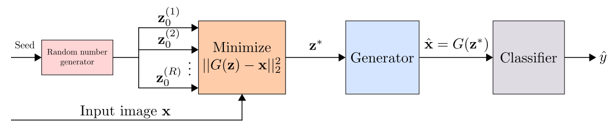
\includegraphics[scale = 0.9]{Figures/figura_32.PNG}
\decoRule
\caption[Redes generativas con adversario (GAN) como defensas]{Redes generativas con adversario (GAN) como defensas \parencite{r39}.}
\label{fig:32}
\end{figure}

Esta defensa pretende ser efectiva tanto a ataques de caja blanca o caja negra. Su desventaja es que baja la efectividad de clasificación del modelo.


\section{Destilación como defensa}

Dentro de las técnicas de protección, existe una categoría en la cual se realiza un enmascaramiento de gradientes. La mayoría de los ataques de caja blanca operan computando gradientes del modelo y, por lo tanto, fallan si es imposible calcular gradientes útiles. El enmascaramiento de gradiente consiste en hacer que el gradiente sea inútil, ya sea cambiando el modelo de alguna manera que lo hace imperceptible o que tenga gradiente cero en la mayoría de los lugares.
La destilación es una técnica de entrenamiento formulada para transferir conocimiento de un modelo de aprendizaje profundo a otro, con el fin de reducir la complejidad computacional transfiriendo el conocimiento de arquitecturas más grandes a arquitecturas más pequeñas \parencite{r61}. Estudios recientes propusieron una variante de dicha técnica como defensa frente a ejemplos adversarios, en donde se utiliza el conocimiento extraído de un modelo para mejorar su propia robustez. en donde se entrena al clasificador en dos rondas. La figura~\ref{fig:33} muestra el proceso de destilación, en donde se entrena una red de como comúnmente se hace, y luego se utiliza su vector de predicción como etiqueta en una segunda red para cada dato de entrenamiento. Esto tiene el efecto de generar una red más fluida y reducir la amplitud de los gradientes alrededor de los puntos de entrada, lo que dificulta que los atacantes generen ejemplos adversarios \parencite{r24}. Si los gradientes son altos, la elaboración de ejemplos adversarios es más fácil porque pequeñas perturbaciones inducen altas variaciones en la clasificación del modelo. 
Si bien la destilación defensiva es eficaz en ataques de caja blanca, no protege adecuadamente contra los ataques de caja negra con ejemplos adversarios transferidos desde otro modelo \parencite{r28}. Por otra parte, este tipo de defensa sólo es eficaz frente a ataques que se formulan a partir del gradiente descendiente, siendo aún vulnerable a otros tipos de ataques, como por ejemplo, los realizados por regresión de los modelos como se expuso en estudios posteriores \parencite{r55}. 

\begin{figure}[th]
\centering
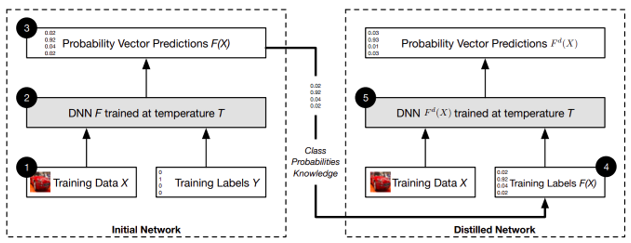
\includegraphics[scale = 0.9]{Figures/figura_33.PNG}
\decoRule
\caption[Entrenamiento con técnica de destilación ) como defensas]{Entrenamiento con técnica de destilación como defensa \parencite{r24}.}
\label{fig:33}
\end{figure}

\section{Agregar la clasificación NULL}

Otra técnica de protección consiste en agregar una nueva salida de la red llamada NULL, en la cual se entrena la red para que pueda clasificar los ejemplos adversarios en esta categoría. La figura~\ref{fig:34} muestra cómo opera este método de defensa con imágenes del conjunto de datos MNIST. La imagen superior (dígito cero) corresponde a la original, mientras que las inferiores son ejemplos adversarios. En la figura se compara un clasificador tradicional versus cómo clasifica el modelo con la salida NULL. cuando la clase NULL toma valores por sobre cierto valor (a determinar en cada modelo) es posible detectar un ataque. Este mecanismo de defensa es efectivo frente a los ataques del tipo caja negra, ya que rompe la transferibilidad de los ejemplos adversarios \parencite{r7} al agregar la nueva clase NULL al modelo. La desventaja de este mecanismo es que baja la efectividad de clasificación del modelo.


\begin{figure}[th]
\centering
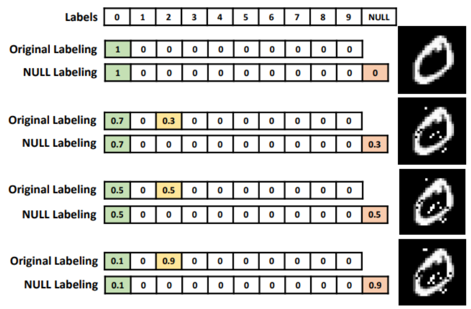
\includegraphics{Figures/figura_34.PNG}
\decoRule
\caption[Clasificación NULL de ejemplos adversarios]{Clasificación NULL de ejemplos adversarios \parencite{r7}.}
\label{fig:34}
\end{figure}

\section{Arquitectura de software resiliente}
Un estudio reciente de la Scuola Superiore Sant’Anna, Pisa \parencite{r5}, proponen un modelo para brindar seguridad a los sistemas de aprendizaje profundo desde la mirada de la arquitectura de software, apuntando principalmente a los sistemas críticos, con objetivos como robustez, tolerancia a fallos y lo más certificable posible, ya que su mal funcionamiento en este tipo de sistema podría poner en riesgo vidas humanas o desatar un desastre medio ambiental. Además, en los sistemas críticos deben reaccionar a los eventos en un tiempo predecible. Una salida de control entregada demasiado tarde podría ser inútil o incluso peligroso (como ejemplo, un comando de frenado en un auto con conducción automática). Esto significa que estos sistemas deben ser verificables no solo en el dominio funcional, sino también en el dominio del tiempo. El estudio propone un sistema de alta disponibilidad de clúster de servidores. Este sistema puede ser activo-pasivo o activo-activo, dependiendo de cómo se requiera administrar los recursos. 
Una de las dificultades que existen en certificar como sistema crítico un sistema de aprendizaje profundo es en cuanto a lo siguiente:
\begin{itemize}
    \item Los resultados obtenidos de una red neuronal artificial no son 100\% confiables. 
    \item Los sistemas basados en redes neuronales artificiales comúnmente son desarrollados usando marcos de trabajos como TensorFlow, Keras o Caffe que facilitan su implementación, permitiendo crear modelos óptimos de redes neuronales con pocas líneas de código. Estos no son compatibles con el estándar de codificación usado en certificaciones de sistemas de software críticos. 
    \item Estos sistemas generalmente se ejecutan en sistemas operativos como Linux, los cuales no son sistemas operativos de tiempo real, comúnmente usados en sistemas críticos.
\end{itemize}
En estos sistemas se hace necesario contar con este dominio no certificable, ya que los controladores de dispositivo (como la GPU) y software necesarios para la operaciones de una red neuronal artificial solo están disponibles para sistemas operativos enriquecidos, y no de tiempo real utilizados y exigido por certificaciones de sistemas críticos. Para poder resolver estas desventajas el estudio propone la arquitectura presentada en la figura~\ref{fig:35}, la cual posee un dominio de software no certificable en los estándares de sistemas críticos, que se compone de 3 modelos de redes neuronales distintos (aunque pudiesen ser más) que clasifican en paralelo las entradas, los cuales se ejecutan en servidores independientes con sistemas operativos enriquecidos (ejemplo Linux). También cuenta con una máquina con sistema operativo de tiempo real (RTOS) que cumple funciones de control, monitoreo y consolidación de los resultados obtenidos por los modelos de redes neuronales artificiales llamado “Dominio crítico” que posee infraestructura y software certificable. Además, incluye una capa que cumple la función de hipervisor de estas máquinas, monitoreando disponibilidad y seguridad. El Hipervisor si detecta un comportamiento no esperado en las máquinas de SO puede ejecutar procedimientos de recuperación. La infraestructura y software del Hypervisor es certificable.

\begin{figure}[th]
\centering
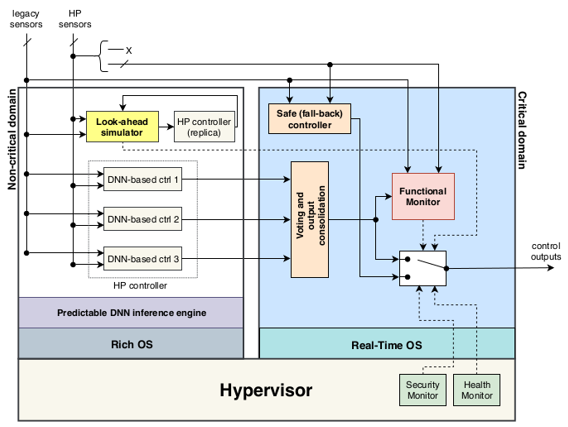
\includegraphics{Figures/figura_35.PNG}
\decoRule
\caption[Arquitectura para redes neuronales artificiales en sistemas críticos]{Arquitectura para redes neuronales artificiales en sistemas críticos \parencite{r5}.}
\label{fig:35}
\end{figure}

\subsection{Consideraciones adicionales de seguridad}
A continuación se presentan algunas consideraciones de seguridad a tener en cuenta al implementar una red neuronal artificial:
\begin{itemize}
    \item \textbf{Datos de entrenamiento confiables:} Para evitar ataques como los del tipo envenenamiento de datos se ha de tener precaución en cuanto al origen de los datos de entrenamiento. Dependiendo de la criticidad en la cual operará el sistema, se podría evaluar generar datos de prueba propios. Si esto no fuese factible, otra opción es chequear los conjunto de datos con algún otro modelo.
    \item \textbf{Restringir accesos al modelo:} El acceso a el modelo de la red neuronal artificial debe estar habilitado solo para personal autorizado, como también la documentación, datos de entrenamiento, parámetros y topología. Solo deben ser expuestas las interfaces de entrada y salida a los demás usuarios.  
    \item \textbf{Resultados específicos:} Si es posible, la salida restringirla sólo al atributo clasificado de forma booleana, sin indicar los porcentajes, para evitar la extracción del modelo.

\end{itemize}
